\newcommand{\svcourse}{CST Part IA: Introduction to Probability}
\newcommand{\svnumber}{1}
\newcommand{\svvenue}{Churchill, Room TBD}
\newcommand{\svdate}{2022-05-14}
\newcommand{\svtime}{11:00}
\newcommand{\svuploadkey}{PO5ogKIM8KQA22FZS8IAf8gxA8XKi19jxIBVHIfFZ+3GCBXuNUXS9lVN6bNYjxM/}

\newcommand{\svrname}{Mr Matthew Ireland}
\newcommand{\jkfside}{twoside}
\newcommand{\jkfhanded}{right}

\newcommand{\studentname}{Harry Langford}
\newcommand{\studentemail}{hjel2@cam.ac.uk}


\documentclass[10pt,\jkfside,a4paper]{article}

\input{../../template/includes.tex}
% DO NOT add \usepackage commands here.  Place any custom commands
% into your SV work files.  Anything in the template directory is
% likely to be overwritten!

\usepackage{fancyhdr}

\usepackage{lastpage}       % ``n of m'' page numbering
\usepackage{lscape}         % Makes landscape easier

\usepackage{verbatim}       % Verbatim blocks
\usepackage{epsfig}         % Embed encapsulated postscript
\usepackage{array}          % Array environment
\usepackage[nolinks]{qrcode}         % QR codes
\usepackage{enumitem}       % Required by Tom Johnson's exam question header

\usepackage{hhline}         % Horizontal lines in tables
\usepackage{siunitx}        % Correct spacing of units
\usepackage{amsmath}        % American Mathematical Society
\usepackage{amssymb}        % Maths symbols
\usepackage{amsthm}         % Theorems

\usepackage{ifthen}         % Conditional processing in tex

\usepackage[top=3cm,
            bottom=3cm,
            inner=2cm,
            outer=5cm]{geometry}

% PDF metadata + URL formatting
\usepackage[
            pdfauthor={\studentname},
            pdftitle={\svcourse, SV \svnumber},
            pdfsubject={},
            pdfkeywords={9d2547b00aba40b58fa0378774f72ee6},
            pdfproducer={},
            pdfcreator={},
            hidelinks]{hyperref}

\renewcommand{\headrulewidth}{0.4pt}
\renewcommand{\footrulewidth}{0.4pt}
\fancyheadoffset[LO,LE,RO,RE]{0pt}
\fancyfootoffset[LO,LE,RO,RE]{0pt}
\pagestyle{fancy}
\fancyhead{}
\fancyhead[LO,RE]{{\bfseries \studentname}\\\studentemail}
\fancyhead[RO,LE]{{\bfseries \svcourse, SV~\svnumber}\\\svdate\ \svtime, \svvenue}
\fancyfoot{}
\fancyfoot[LO,RE]{For: \svrname}
\fancyfoot[RO,LE]{\today\hspace{1cm}\thepage\ / \pageref{LastPage}}
\fancyfoot[C]{\qrcode[height=0.8cm]{\svuploadkey}}
\setlength{\headheight}{22.55pt}

\ifthenelse{\equal{\jkfside}{oneside}}{

 \ifthenelse{\equal{\jkfhanded}{left}}{
  % 1. Left-handed marker, one-sided printing or e-marking, use oneside and...
  \evensidemargin=\oddsidemargin
  \oddsidemargin=73pt
  \setlength{\marginparwidth}{111pt}
  \setlength{\marginparsep}{-\marginparsep}
  \addtolength{\marginparsep}{-\textwidth}
  \addtolength{\marginparsep}{-\marginparwidth}
 }{
  % 2. Right-handed marker, one-sided printing or e-marking, use oneside.
  \setlength{\marginparwidth}{111pt}
 }

}{
 % 3. Alternating margins, two-sided printing, use twoside.
}

\setlength{\parindent}{0em}
\addtolength{\parskip}{1ex}

% Exam question headings, labels and sensible layout (courtesy of Tom Johnson)
\setlist{parsep=\parskip, listparindent=\parindent}
\newcommand{\examhead}[3]{\section{#1 Paper #2 Question #3}}
\newenvironment{examquestion}[3]{
    \examhead{#1}{#2}{#3}\setlist[enumerate, 1]{label=(\alph*)}\setlist[enumerate, 2]{label=(\roman*)}
    \marginpar{\qrcode{https://www.cl.cam.ac.uk/teaching/exams/pastpapers/y#1p#2q#3.pdf}}
    \marginpar{\footnotesize \url{https://www.cl.cam.ac.uk/teaching/exams/pastpapers/y#1p#2q#3.pdf}}
}{}



\usepackage{graphicx}
\graphicspath{ {./images/} }
\usepackage{tikz}

\begin{document}

\begin{examquestion}{2013}{2}{3}

Consider a single processor system in which multiple processes are running.

\begin{enumerate}

\item What does it mean for a process to be I/O bound? What does it mean for it to be CPU bound?

A process is I/O bound if the process spends more time waiting for inputs and giving outputs than it 
does processing. This happens when there are a lot of short CPU bursts.

A process is CPU bound if the majority of the time of the process is spent processing data 
rather than inputting or outputting data. In this case CPU bursts are very long.

\item What is the difference between preemptive and non-preemptive scheduling? Which one requires 
specific hardware support and what is that hardware support?

A preemptive scheduling algorithm changes tasks when they are midway through execution. This is usually 
because either the process has passed its allotted amount of time or a higher priority process has arrived -- 
such as an interrupt.

A non-preemptive scheduling algorithm does not change tasks before the task yields control or finishes. 

Preempting scheduling requires hardware support for context switches. To do a context switch we need 
to save the current state of the executing process; write it all to memory and then load the state of 
the next process into the registers. This is computationally expensive and without hardware support 
can outweigh the benefit from a better scheduling algorithm. For example if a CPU has multiple 
registers then context switching could simply be changing a bit pointing to which register the 
CPU is currently using -- or could be done in parallel with normal code execution (ie register set 1 is 
copied by hardware while the CPU uses register set 2).

\item Two processes, $A$ and $B$, have the following sequential execution patterns:

$A$: [cpu 4 ms; I/O 2 ms; cpu 4 ms; I/O 2 ms; cpu 4 ms]\\
$B$: [cpu 1 ms; I/O 2 ms; cpu 1 ms; I/O 2 ms; cpu 1 ms]\\

I/O operations for the two processes do not interfere with each other and are
blocking.

\begin{enumerate}

\item  If the processes are run consecutively one after another, what is the elapsed
time for all to complete?

23ms

\item Sketch the execution pattern under non-preemptive scheduling and
determine the total elapsed time for completion. You may assume that
processes are scheduled in the order in which they become ready to run
and that in the event of a tie $A$ has priority over $B$. You may further
assume that the scheduler and context switches take negligible time.

In non-preemptive scheduling, $A$ has higher priority than $B$ and so $A$ 
starts execution. This is not changed since the scheduler is non-preemptive.

I was unsure what ``execution pattern'' meant. I have therefore made two diagrams 
one for either of the interpretations.

\begin{center}
\includegraphics[width=120mm]{utilisation}
\end{center}

\begin{center}
\begin{tikzpicture}
\filldraw [fill=lightgray!20] (0, 0) rectangle (8.8, 1);
\draw (6.121739130434783, 0) -- (6.121739130434783, 1);
\node [anchor=center] at (3.0608695652173914, 0.5) {$A$};
\node [anchor=center] at (7.460869565217392, 0.5) {$B$};
\draw (0, 0) -- (0, -0.1);
\draw (6.121739130434783, 0) -- (6.121739130434783, -0.1);
\draw (8.8, 0) -- (8.8, -0.1);
\node [anchor=north] at (0, -0.05) {0};
\node [anchor=north] at (6.121739130434783, -0.05) {16};
\node [anchor=north] at (8.8, -0.05) {23};
\end{tikzpicture}
\end{center}

\item Repeat (c)(ii) but for a preemptive scheduler that operates on a time slice
of 2 ms, that is, no process can run for more than 2 ms at a time (unless
no other process is runnable).

\begin{center}
\includegraphics[width=120mm]{utilisationpart2}
\end{center}

\begin{center}
\begin{tikzpicture}
\filldraw [fill=lightgray!20] (0, 0) rectangle (8.8, 1);
\draw (0.8, 0) -- (0.8, 1);
\draw (1.6, 0) -- (1.6, 1);
\draw (2.4, 0) -- (2.4, 1);
\draw (3.2, 0) -- (3.2, 1);
\draw (4.0, 0) -- (4.0, 1);
\draw (4.8, 0) -- (4.8, 1);
\node [anchor=center] at (0.4, 0.5) {$A$};
\node [anchor=center] at (2.0, 0.5) {$A$};
\node [anchor=center] at (3.6, 0.5) {$A$};
\node [anchor=center] at (6.4, 0.5) {$A$};
\node [anchor=center] at (1.2, 0.5) {$B$};
\node [anchor=center] at (2.8, 0.5) {$B$};
\node [anchor=center] at (4.4, 0.5) {$B$};
\draw (0, 0) -- (0, -0.1);
\draw (0.8, 0) -- (0.8, -0.1);
\draw (1.6, 0) -- (1.6, -0.1);
\draw (2.4, 0) -- (2.4, -0.1);
\draw (3.2, 0) -- (3.2, -0.1);
\draw (4.0, 0) -- (4.0, -0.1);
\draw (4.8, 0) -- (4.8, -0.1);
\draw (8.8, 0) -- (8.8, -0.1);
\node [anchor=north] at (0, -0.05) {0};
\node [anchor=north] at (0.8, -0.05) {2};
\node [anchor=north] at (1.6, -0.05) {4};
\node [anchor=north] at (2.4, -0.05) {6};
\node [anchor=north] at (3.2, -0.05) {8};
\node [anchor=north] at (4.0, -0.05) {10};
\node [anchor=north] at (4.8, -0.05) {12};
\node [anchor=north] at (8.8, -0.05) {22};
\end{tikzpicture}
\end{center}

\item Is there any evidence from your results for (c)(ii) and (c)(iii) of a significant
advantage for either scheduling method?

Although the total time taken for both methods is comparable, there is evidence of a significant 
advantage for the preemptive scheduling method. The throughput of the preemptive scheduler 
was marginally higher than that of the non-preemptive scheduler. The waiting time 
was also lower: process $B$ finished before process $A$ did in the non-preemptive scheduler 
and process $A$ finished before process $B$ did in the non-preemptive scheduler. The response time 
was higher since processes were addressed sooner.

However, the preemptive scheduling required significantly more context switches than the 
non-preemptive and had a higher turnaround time than the non-preemptive scheduler.

However, I believe that the first points outweigh the later and so the preemptive scheduler 
was significantly better than the non-preemptive scheduler.

\end{enumerate}

\end{enumerate}

\end{examquestion}

\begin{examquestion}{2012}{2}{3}

\begin{enumerate}

\item To switch between processes, an operating system must save the context of the
current executing process and restore the context of that being resumed.

\begin{enumerate}

\item  By what mechanism is the point of execution of a process preserved and
restored?

We perform a context switch, saving the state of the CPU (including data indicating 
the point of execution) into a PCB.

\item  Describe two methods by which the contents of a process address space are
preserved and restored.

Firstly we could mark the address space as full and simply not use that part of RAM 
until we return to the program and then keep pointers to the address space in the program 
so we can immediately return to it when the process re-enters the running state.

Alternatively we could copy the contents of the process address space into a PCB. This 
frees up space however requires copying across large amounts of data and is very slow.

\item Give two other elements of process context.

Contents of registers and state of the CPU execution (user or kernel mode).

\end{enumerate}

\item The diagram below is a simplified state transition diagram for a process in a
generic operating system.
\begin{center}
\includegraphics{stategeneric}
\end{center}
For each of the following, describe the transitions taken by the process and say
whether or not it is necessary for the process scheduler to run:

\begin{enumerate}

\item A running process is interrupted by a timer. The timer interrupt service
routine determines that the time slice given to the process has not yet
expired.

The timer interrupts the process. So the process enters the interrupted state. 
However since the time slice has not expired then the process can re-enter the 
running state without entering the ready or waiting states.

running $\longrightarrow$ interrupted $\longrightarrow$ running

It is not need to \textit{run} the process scheduler since the process 
should still be executing.

\item As in (b)(i) but the time slice given to the process has expired.

The process will first be interrupted by the timer. So the process enters the 
interrupted state. The timer will establish that the time quantum has expired 
and so place the process into the ready queue (not the waiting queue since the 
process is not waiting on 
anything and could resume execution whenever required).

running $\longrightarrow$ interrupted $\longrightarrow$ ready

It is necessary for the process scheduler to run since the original process 
is not running we must find another process to run. 

\item A running process makes a system call which can be serviced immediately
by the kernel.

The system makes a kernel call. This swaps from running into kernel mode. Since the 
system call can be serviced immediately, it does not need to switch from kernel to 
waiting.

running $\longrightarrow$ kernel

Upon completion of kernel execution we will restore the program to the running state.

It is not necessary for the process scheduler to run.

\item A running process makes a system call which requires an I/O operation to
be initiated.

When we make a system call we must swap to kernel execution. Since the process requires an I/O 
operation, it will enter the waiting state while waiting for user input.

running $\longrightarrow$ kernel $\longrightarrow$ waiting

It could be necessary for the process scheduler to run. If the process yields when 
it starts waiting for the I/O operation then the process scheduler will need to run. 
Otherwise it will not.

\end{enumerate}

\end{enumerate}

\end{examquestion}

\begin{examquestion}{2010}{2}{3}

\begin{enumerate}

\item Shortest Job First (SJF), Shortest Remaining Time First (SRTF) and Round
Robin (RR) are CPU scheduling algorithms. Briefly describe each.

In Shortest Job First, the OS finds the job which it estimates will take the least time to complete 
and then executes it fully. This is a non-preemptive algorithm.

Shortest Remaining Time First will execute the job which it believes will finish in the least time. 
This is different to Shortest Job First since SRTF is preemptive and will change which job it is 
doing if a new job comes which the OS thinks will take less time to execute to completion than the 
job it is currently executing.

Round Robin executes each ojb for a given time quantum and after a job has had that time quantum it 
will move into the waiting state and another job will start executing for it's time quantum.
Round Robin is preemptive.

\item Consider the following set of processes.
\begin{center}
\begin{tabular}{c c c}
Process & Creation Time & Required Computing Time \\
\hline
$P_1$	& 0				& 25\\
$P_2$	& 5				& 15\\
$P_3$	& 10			& 5\\
$P_4$	& 15			& 5\\
\hline
\end{tabular}
\end{center}

\begin{enumerate}

\item  Draw a diagram showing how SJF would schedule the processes. What is
the average waiting time?

\begin{tabular}{c|ccccccccccc}
Time & 0-5 & 5-10 & 10-15 & 15-20 & 20-25 & 25-30 & 30-35 & 35-40 & 40-45 & 45-50 \\
\hline
Arrival & $P_1$ & $P_2$ & $P_3$ & $P_4$ & & & & & \\
Process & $P_1$ & $P_1$ & $P_1$ & $P_1$ & $P_1$ & $P_3$ & $P_4$ & $P_2$ & $P_2$ & $P_2$ \\
\end{tabular}

The average waiting time is the sum of the times that each process spent in the ready state waiting for 
CPU time divided by the number of processes.
\begin{equation*}
\begin{split}
\overline{W} &= \frac{\sum^n_{i=0} W_i}{n}\\
\overline{W} &= \frac{0s + 25s + 30s + 35s}{4}\\
\overline{W} &= \frac{90s}{4}\\
\overline{W} &= 22.5s\\
\end{split}
\end{equation*}

\item  Draw a diagram showing how SRTF would schedule the processes. What
is the average waiting time in this case?

\begin{tabular}{c|ccccccccccc}
Time & 0-5 & 5-10 & 10-15 & 15-20 & 20-25 & 25-30 & 30-35 & 35-40 & 40-45 & 45-50 \\
\hline
Arrival & $P_1$ & $P_2$ & $P_3$ & $P_4$ & & & & & \\
Process & $P_1$ & $P_2$ & $P_3$ & $P_4$ & $P_2$ & $P_2$ & $P_1$ & $P_1$ & $P_1$ & $P_1$ \\
\end{tabular}
\begin{equation*}
\begin{split}
\overline{W} &= \frac{\sum^n_{i=1} W_i}{n}\\
\overline{W} &= \frac{(0s + 25s) + (0s + 10s) + 0s + 0s}{4}\\
\overline{W} &= \frac{35s}{4}\\
\overline{W} &= 8.75s\\
\end{split}
\end{equation*}

\item Assuming a quantum of 10 time units, draw a diagram showing how RR
would schedule the processes. What is the average waiting time in this
case?

\begin{tabular}{c|ccccccccccc}
Time & 0-5 & 5-10 & 10-15 & 15-20 & 20-25 & 25-30 & 30-35 & 35-40 & 40-45 & 45-50 \\
\hline
Arrival & $P_1$ & $P_2$ & $P_3$ & $P_4$ & & & & & \\
Process & $P_1$ & $P_1$ & $P_2$ & $P_2$ & $P_3$ & $P_4$ & $P_1$ & $P_1$ & $P_2$ & $P_1$ \\
\end{tabular}
\begin{equation*}
\begin{split}
\overline{W} &= \frac{\sum^n_{i=1} W_i}{n}\\
\overline{W} &= \frac{(0s + 20s + 5s) + (5s + 20s) + 10s + 10s}{4}\\
\overline{W} &= \frac{70s}{4}\\
\overline{W} &= 17.5s\\
\end{split}
\end{equation*}

\item A student suggests that RR could be improved by reducing the quantum
to 1 time unit. What are the advantages and disadvantages of this
proposal?

There are a few small advantages of this method: firstly since we only use quanta of size 1, 
this is very simple to implement (both for the programmer and for the CPU). So there will 
be very little scheduling overhead.

Furthermore, since we are swapping every time unit, we are guaranteed that a process will 
finish quickly. So short Jobs are guaranteed to finish sooner and will not be stuck in the 
waiting queue for extended periods of time. This ``one-quantum Round Robin'' could also 
beat Shortest Job First or Shortest Remaining Time First if there are bad estimates for 
the amount of time a job will take since we make no assumptions about time requirement 
using this scheduling method. We are also guaranteed never to be held up by IO-bound jobs. 
This theoretically maximises CPU utilisation. However there are better strategies to 
maximise CPU utilisation which do not involve such a high amount of context switches.

However, in comparison to the advantages, the disadvantages are numerous and more meaningful. 

The most obvious disadvantage is that we require a context switch every time unit. In 
theoretical computer science this will have hardware support and the time requirement 
will be negligible. However in all practical applications there will be a severe overhead 
for each context switch -- context switching every quantum will lead to threshing: the CPU 
will spend more time switching processes than executing. This is suboptimal.

Secondly we do not prioritise any type of jobs. Under this execution method a high-priority 
interrupt or other high-priority task may come across requiring $\geq$ 1 quantum to execute. 
Under this model it would be treated like any other task and would not be accessed quickly. 
In more realistic examples since we do not prioritise any specific tasks we will end up with 
high latency (the mouse response for example may take more than one quantum and so would 
have to wait multiple cycles). Following on from this point, we do not prioritise shorter 
tasks and so the amount of tasks in the waiting queue will be higher than other scheduling 
algorithms.

While we do not run the risk of process starvation, we penalise long tasks -- they will have 
to execute one quantum at a time and so perhaps wait for hundreds or thousands of cycles.
While this strategy minimises waiting time; it maximises turnaround time.

Overall I believe that using a time quantum of 1 for Round Robin is not a great idea. We 
would be better selecting a time quantum which would make Round Robin conform the the 80-20 rule 
(wherein $\sim80\%$ of processes take less than one time quantum but $\sim20\%$ do not)

\end{enumerate}

\end{enumerate}

\end{examquestion}

\end{document}